\chapter{\MakeUppercase{Project Implementation}}
\section{Implementation Overview}
The project is implemented in Python. The file \verb|environment.py| defines the disaster \ac{dtn} testbed, simulation constants, node creation, message generation, mobility update, contact detection, delivery checking, expiration, and metric computation. The file \verb|message.py| defines message identity, source, destination, creation time, critical flag, hop count, and copy count. The file \verb|node.py| defines node identity, role, mobility properties, location, and buffer.

The routing implementations are placed inside the \verb|routing| package. The baselines are implemented in \verb|routing/epidemic.py| and \verb|routing/spray.py|. The proposed protocol is implemented in \verb|routing/spatio_semantic.py|. The experiment runner in \verb|main.py| executes every protocol across all traffic levels and writes aggregate outputs to the \verb|plots| directory.

\section{Code Structure and Execution Flow}
The implementation follows the same separation of concerns described in the design chapter. The environment acts as the orchestration layer. It initializes nodes, advances time, invokes the selected routing module during contacts, and records outcome statistics. This keeps the experiment control logic in one place and allows the routing files to focus only on forwarding behavior.

The sequence starts in the file \verb|main.py|. In \verb|main.py|, protocol definitions and traffic patterns to be simulated are set. For every combination of the two, the simulator runs in multiple rounds, and the statistics are collected. When all rounds end, the averages are saved into separate \ac{csv} files for the protocols. The pipeline is thus simple and clear, and the output generated from experiment execution is directly fed into the dashboard via \verb|plots| directory files.

\section{Environment Implementation}
The environment creates four node classes:

\begin{itemize}
	\item 35 civilians with slow movement.
	\item 8 responders with medium movement.
	\item 3 static shelters clustered in one region.
	\item 5 drones with high movement speed.
\end{itemize}

At every time step, the environment probabilistically generates messages, moves nodes, detects contacts, invokes router exchanges, checks deliveries, and removes expired messages. This implementation gives all protocols the same external conditions and isolates differences to their routing decisions.

The environment also acts as the central accounting module. It tracks the number of generated messages, delivered messages, critical deliveries, message delays, transmissions, and buffer drops. Placing these counters inside the environment rather than inside individual routers ensures that the performance metrics are computed consistently. Each router may decide differently, but all routers are judged by the same bookkeeping rules.

\section{Routing Baseline Implementation}
The Epidemic router clones messages to any encountered node that lacks the message. It increments the transmission counter for every successful transfer and increments the drop counter when the receiver buffer is full.

The Spray and Wait router uses message copy counts. When a sender has more than one copy, it gives one copy to a receiver that does not already hold the message. When a message has only one copy, it is forwarded only to the destination. This design reduces unnecessary replication but can also slow delivery.

The implementations of these two baselines are deliberately kept simple. The purpose of their inclusion in the code is not to cover all variations that have been discussed in the literature but rather to demonstrate reference behaviors for Epidemic and Spray-and-Wait. Epidemic allows for unconstrained replication, whereas Spray-and-Wait restricts replication. Given that both these baselines are concise and comprehensible, the impact of our router can be easily analyzed.

\section{Spatio-Semantic Router Implementation}
The router uses two tracking tables per node:

\begin{itemize}
	\item Encounter table: stores the decayed frequency of contact with other nodes.
	\item Zone table: stores the decayed frequency of visits to spatial zones.

\end{itemize}

Both tables are updated during interactions. After that, the router calculates the utility of both sender and receiver to reach the destination node where the message has to be delivered. In case of a match between the receiver and destination nodes, the delivery process takes place immediately. Otherwise, depending on message priority and copy count, the protocol decides to spray, use utility-forward, or wait.

In terms of implementation, the router acts as a contact-time decision maker. Reading the states of the sender, receiver, and message upon contact, the router makes calculations of utility scores and applies certain thresholds that define whether or not the message is sent and how many copies have to be moved. Such design allows keeping the message transfer logic transparent and helps build direct connections between the code execution and algorithm described in the thesis.

\section{Critical Buffer Reserve}
Implementation assigns thirty-five percent of the buffer space to the critical traffic. The remaining percentage of buffer is reserved exclusively for non-critical messages. The critical traffic can use any free slot, even replace non-critical traffic if needed. This way we avoid the situation where the non-critical traffic consumes all the space.

Implementation according to the objective of the thesis is best represented by the reserve policy. Rather than dealing with priority in terms of utility values, the algorithm implements priority during the process of insertion. This is essential since a router may make an appropriate choice of relay for an important packet and yet be unable to keep it safe if the receiving buffer is full of packets having less priority.

\section{Result and Visualization Implementation}
The file \verb|dashboard.py| loads the three result files:

\begin{itemize}
	\item \verb|plots/epidemic_results.csv|
	\item \verb|plots/spray_results.csv|
	\item \verb|plots/spatio_semantic_results.csv|
\end{itemize}

Trend graphing, radar graphing, the display of metrics, and a button for visual simulation are included in the dashboard interface. The \verb|modern_multi_demo.py| file shows a three-pane, full-screen visualization showing Epidemic, Spray \& Wait, and Spatio-Semantic Routing.

This implementation-level tool goes beyond mere presentation. By allowing the generation of plots based on the same metrics used in the analysis, the dashboard serves as an effective bridge between the experimental software and analysis presented in the thesis. This live comparison also makes clear how certain characteristics lead to particular behavior. Congestion, clustering, and mobility make a visual comparison more enlightening than tabular analysis alone.

\section{Implementation Choices for Maintainability}
There have been some implementation decisions made in order to make sure that the maintainability of the project is ensured. The protocol logic has been separated from the environment logic such that any changes to the algorithms do not necessitate changes to the message creation, movement, and calculation of metrics in order to ensure that the project is easily testable and can be extended easily.

It is important to note that maintainability is also important for the credibility of the thesis. This is because there will always be more than one module that interacts in the same application when working on a thesis. Thus, by creating a modular design where different modules have well-defined roles, the implementer is able to conduct experiments as well as report on the work.

\section{Metric Export Workflow}
After each experiment is performed, the collected data points are exported into the plots directory in format-specific output files. The export process is kept simple since these same files will be read later by the dashboard and also referenced in the tables of the thesis. An efficient metric-export pipeline reduces the likelihood of any inconsistency between the simulation results and analysis presented.

The procedure will also allow better repeatability because, if something is altered, running the tests again produces the results in terms of the new \ac{csv} output files and thus eliminates the need for recording the data manually. This way, it will be possible to use the implementation-execution-inspection-revision cycle effectively when comparing several approaches under different traffic loads.

\begin{figure}[h!]
    \centering
    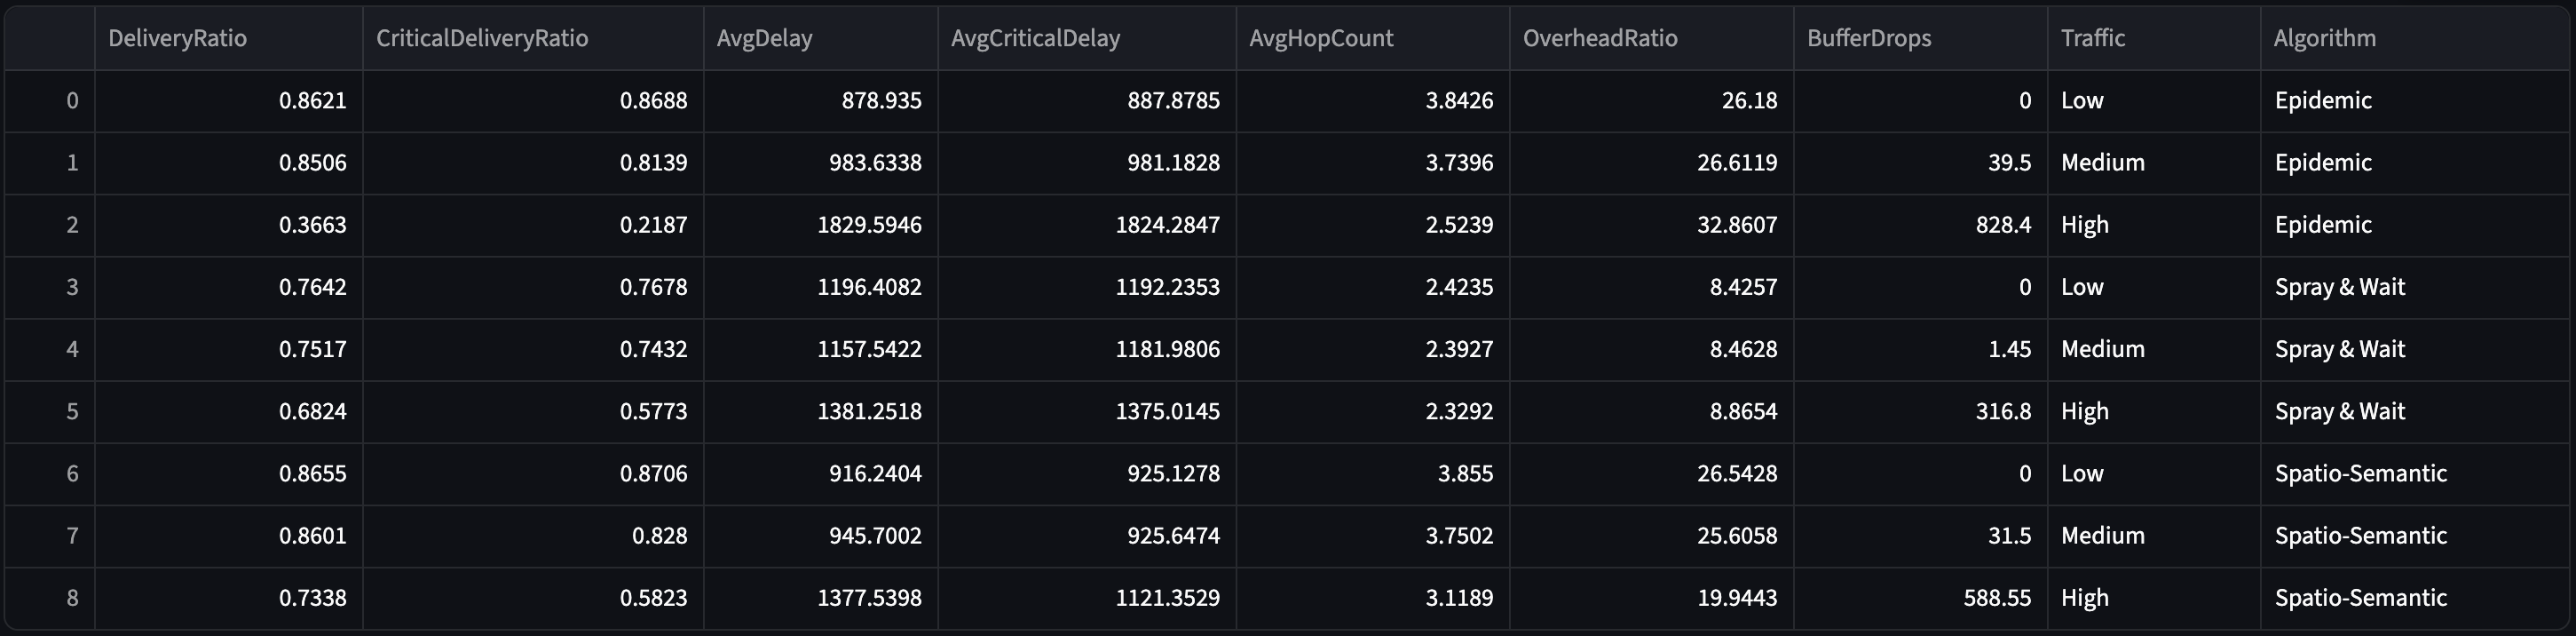
\includegraphics[width=0.85\textwidth]{images/raw-data.png}
    \caption{Raw aggregated simulation results in the dashboard}
    \label{fig:raw_data_placeholder}
\end{figure}
